\section{Рабочий проект}
\subsection{Классы, используемые при разработке сайта}

Можно выделить следующий список классов и их методов, использованных при разработке веб-приложения (таблица \ref{class:table}).

\renewcommand{\arraystretch}{0.8} % уменьшение расстояний до сетки таблицы
\begin{xltabular}{\textwidth}{|X|p{2.5cm}|>{\setlength{\baselineskip}{0.7\baselineskip}}p{4.85cm}|>{\setlength{\baselineskip}{0.7\baselineskip}}p{4.85cm}|}
\caption{Описание классов, используемых в приложении\label{class:table}}\\
\hline \centrow \setlength{\baselineskip}{0.7\baselineskip} Название класса & \centrow \setlength{\baselineskip}{0.7\baselineskip} Модуль, к которому относится класс & \centrow Описание класса & \centrow Методы \\
\hline \centrow 1 & \centrow 2 & \centrow 3 & \centrow 4\\ \hline
\endfirsthead
\caption*{Продолжение таблицы \ref{class:table}}\\
\hline \centrow 1 & \centrow 2 & \centrow 3 & \centrow 4\\ \hline
\finishhead
Validator & Валидатор & Validator - реализует логику валидации и проверки данных, которые намереваются отправить в sql, для поддержания её стабильности & required - проверка наличия значения, type - numeric, date, string, max - ограничение длины строки, pattern - валидация email/телефона, foreign - cуществование в связанной таблице.\\
\hline * & * & * & *
\end{xltabular}
\renewcommand{\arraystretch}{1.0} % восстановление сетки

\newpage 
\subsection{Описание элементов интерфейса пользователя}

На рисунке \ref{index:image} главная страница сайта Pc-Club содержит информацию, навигацию, пример работ.

\begin{enumerate}
	\item Панель навигации.
	\item Переход на страницу админ панели.
	\item Переход на страницу оформления.
	\item Смена учетной записи.
	\item Информационный блок.
	\item Переход к оформлению.
	\item Информационный блок, преимущества Pc-Club.
	\item Блок с примерами работ.
	\item Кастомный скролл.
	\item Footer сайта с информацией.
\end{enumerate}

\begin{figure}[ht]
\center{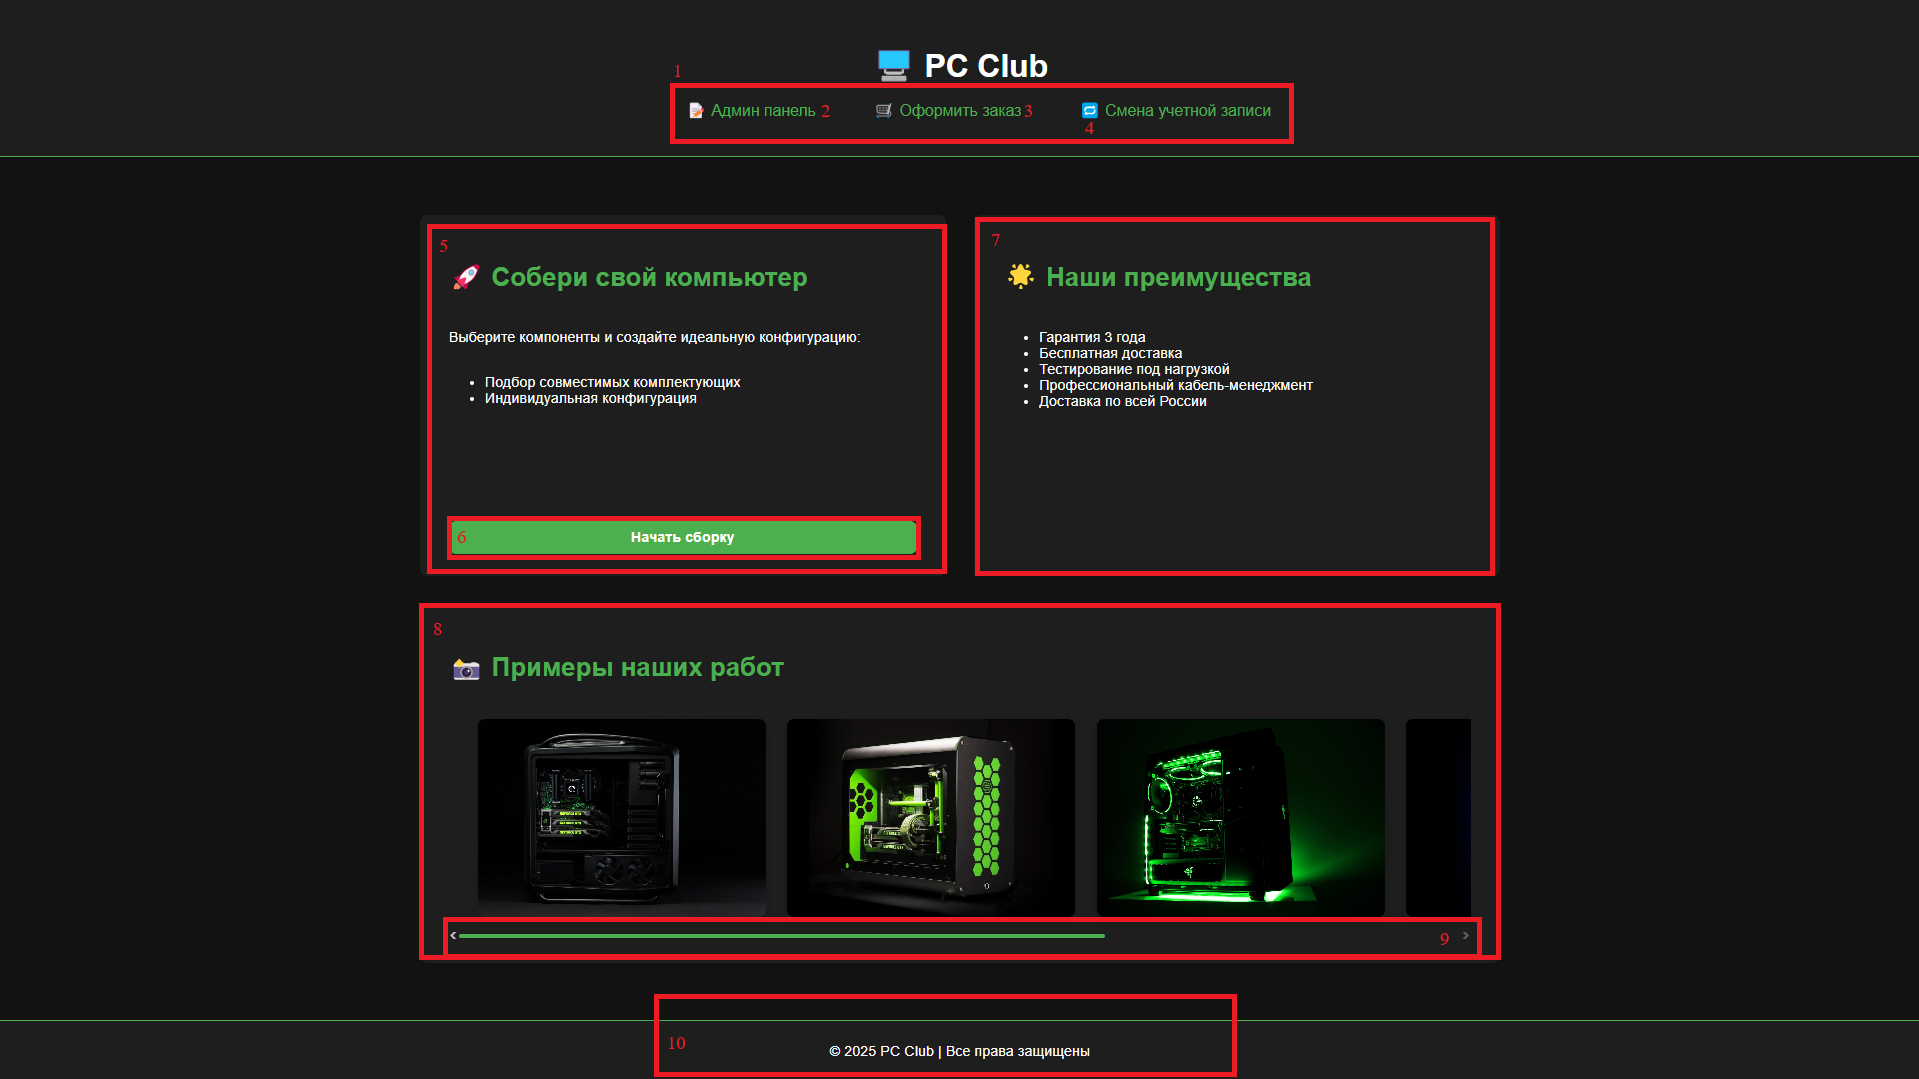
\includegraphics[width=1\linewidth]{index}}
\caption{Главная страница сайта.}
\label{index:image}
\end{figure}

\newpage 
На рисунке \ref{main:image} представлено меню оформления заказа,  в каждом поле можно вписать вручную или выбрать из выпадающего списка.
\begin{enumerate}
	\item Переход на страницу админ панели.
	\item Переход на главную страницу.
	\item Смена учетной записи.
	\item Простая форма ввода только чисел для цены.
	\item Форма ввода с календарем для вывода дат, проверяет на корректность.
	\item Простая форма ввода для адреса.
	\item Выбор из выпадающего списка.
	\item Выбор из выпадающего списка с возможностью ручного ввода.
	\item Кнопка собирает информацию с форм и отправляет в sql.
	\item Выпадающее меню.
	\item Поле ручного ввода/поиска по компонентам в sql.
	\item Кнопка развернуть.
	\item Виды комплектующих из sql.
	\item Сколько этих комплектующих осталось на складе.
\end{enumerate}

\begin{figure}[H]
\center{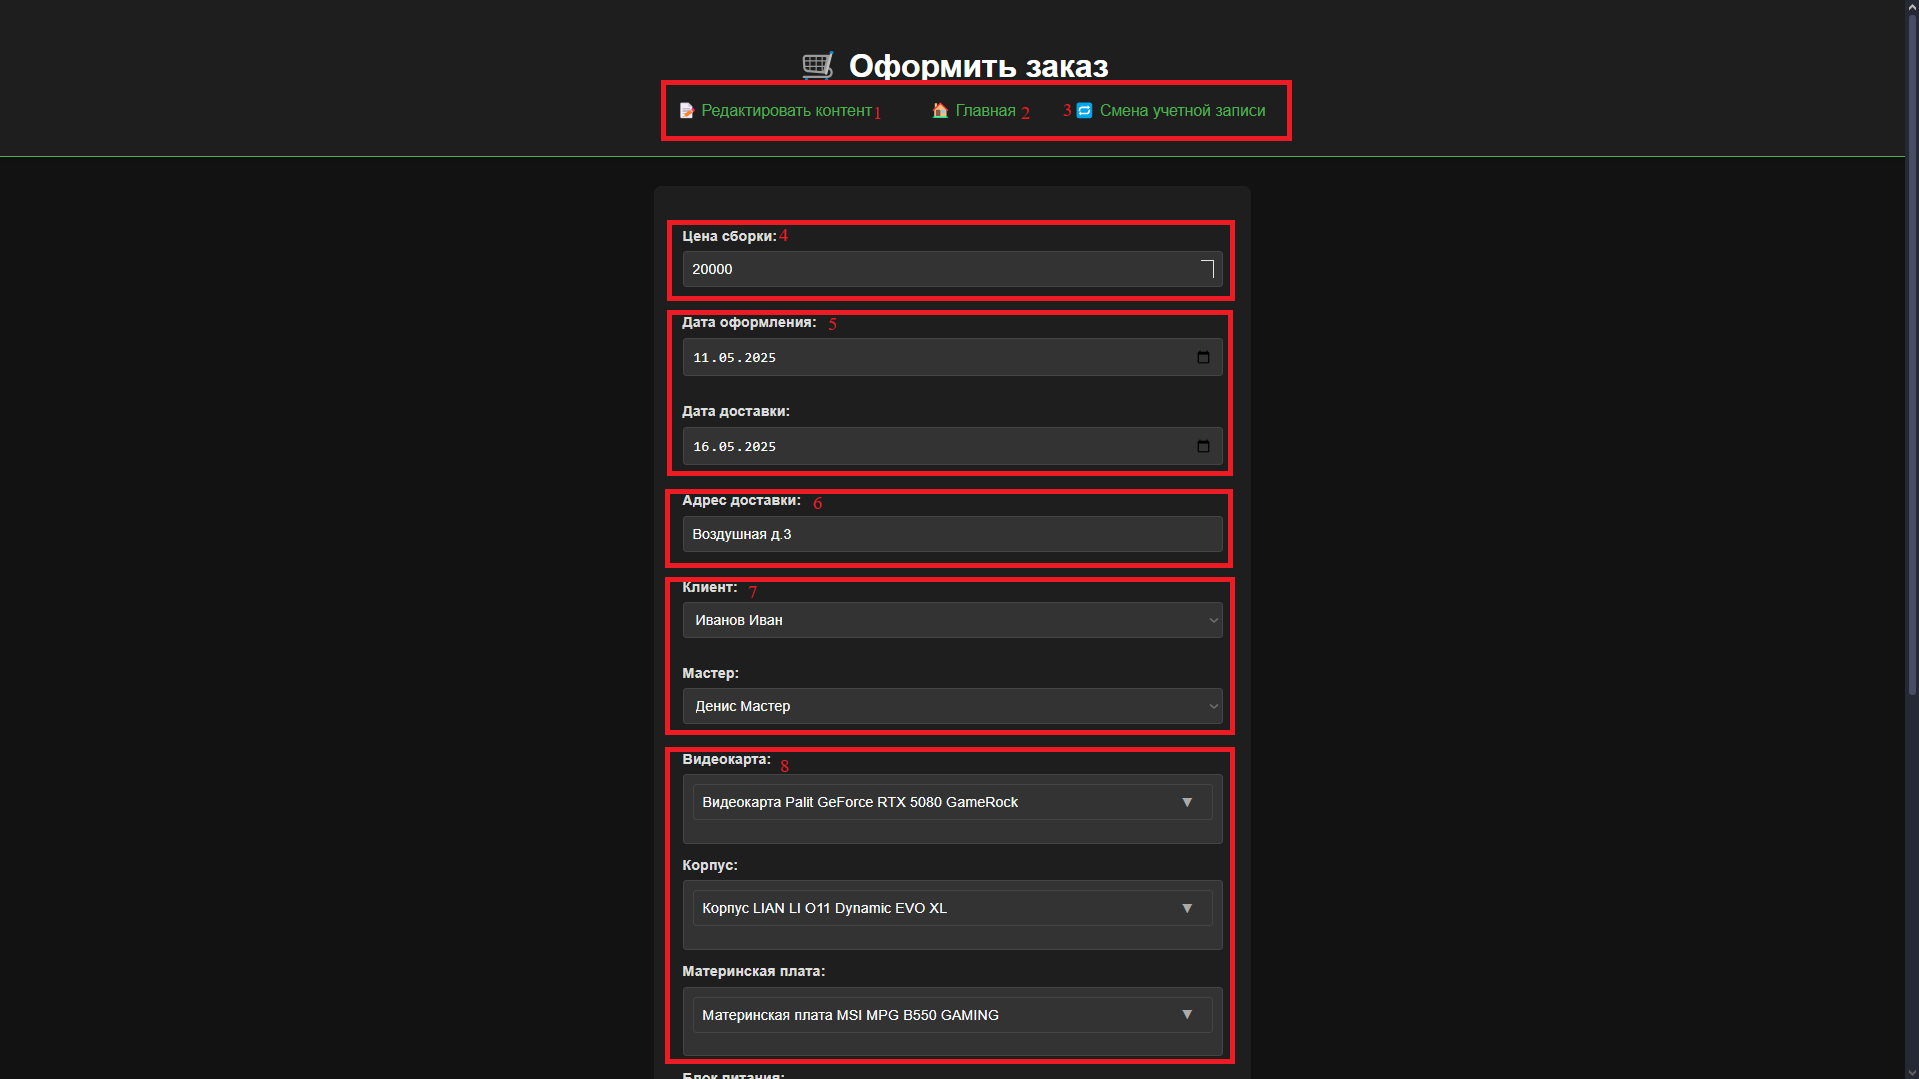
\includegraphics[width=0.9\linewidth]{order+fl}}
\center{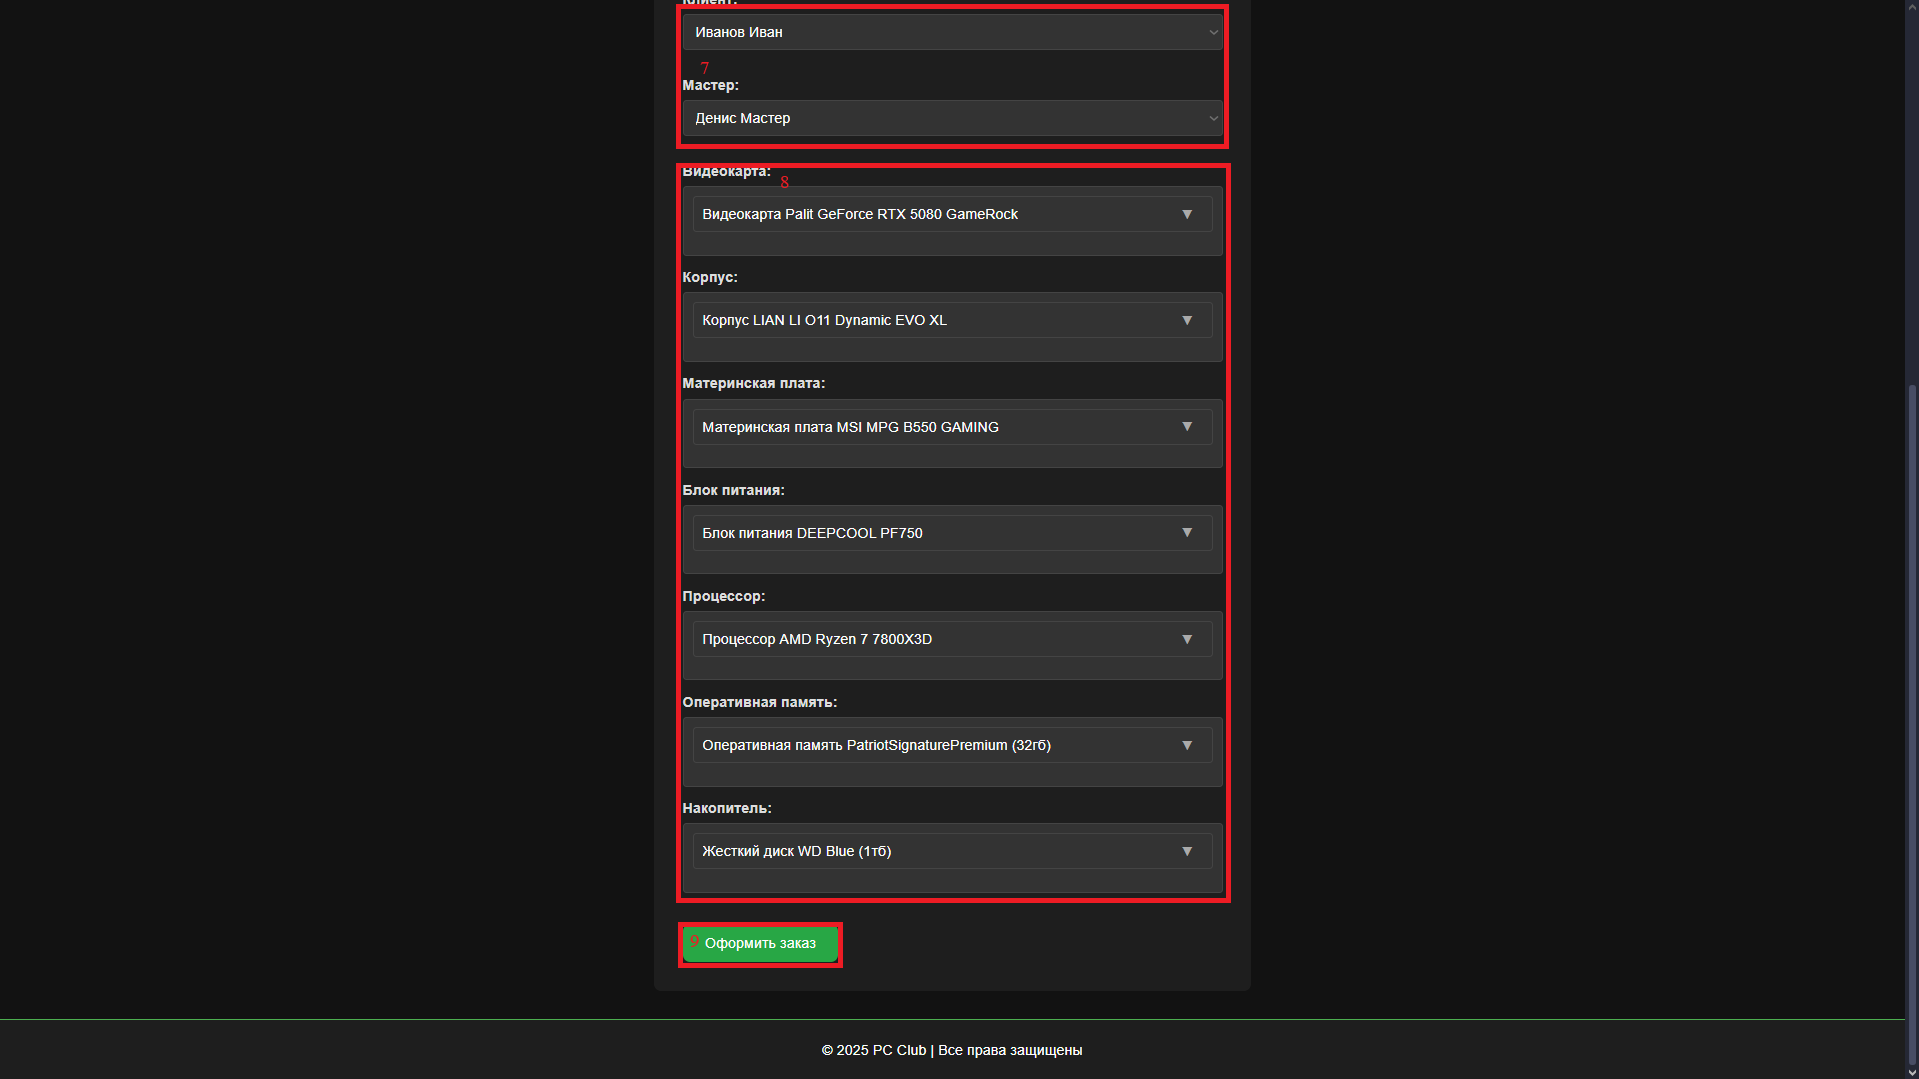
\includegraphics[width=0.9\linewidth]{order+fln}}
\center{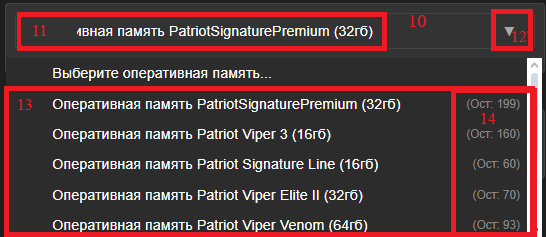
\includegraphics[width=0.75\linewidth]{chosenone}}
\caption{Страница оформления заказа и выпадающее меню компонента.}
\label{main:image}
\end{figure}

На рисунке \ref{login:image} меню для авторизации пользователей в системе, после авторизации под админской учетной записью можно получить доступ к админ панели, складу.
\begin{enumerate}
	\item Форма ввода логина.
	\item Форма ввода пароля.
	\item Кнопка сравнивает логин и хэш пароля с хранящимся в sql, при совпадении пропускает.
	\item Кнопка сохраняет логин и хэш пароля в sql.
	\item Вернуться на главную страницу.
\end{enumerate}
\begin{figure}[ht]
	\center{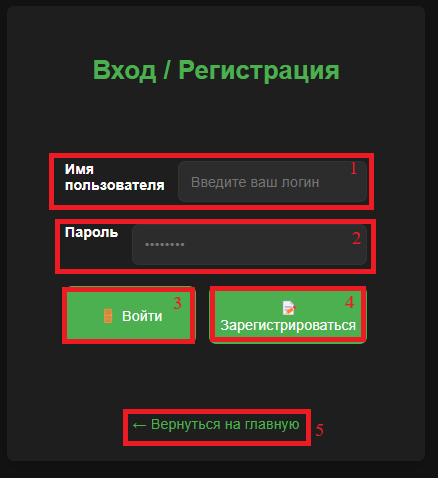
\includegraphics[width=0.25\linewidth]{login}}
	\caption{Разделы для каждого вида компонентов.}
	\label{login:image}
\end{figure}

На рисунке \ref{adminall:image} Панель администратора Pc-Club позволяет полностью контролировать и редактировать информацию в sql.

\begin{enumerate}
	\item Панель навигации по сайту.
	\item Открыть меню выбора компонента.
	\item Ручной поиск по позициям и кнопка.
	\item Добавление новой записи в sql, через админ панель можно напрямую добавить новые компоненты в sql для их дальнейшего использования.
	\item Кнопка для редактирования, можно редактировать любую запись сделаную в таблицы sql.
	\item Кнопка для удаления, удалить любую запись из sql.
	\item Заголовок таблицы, в нашем случае для заказов.
	\item Контент таблицы, хранимый и извлеченный из sql.
\end{enumerate}

\begin{figure}[ht]
\center{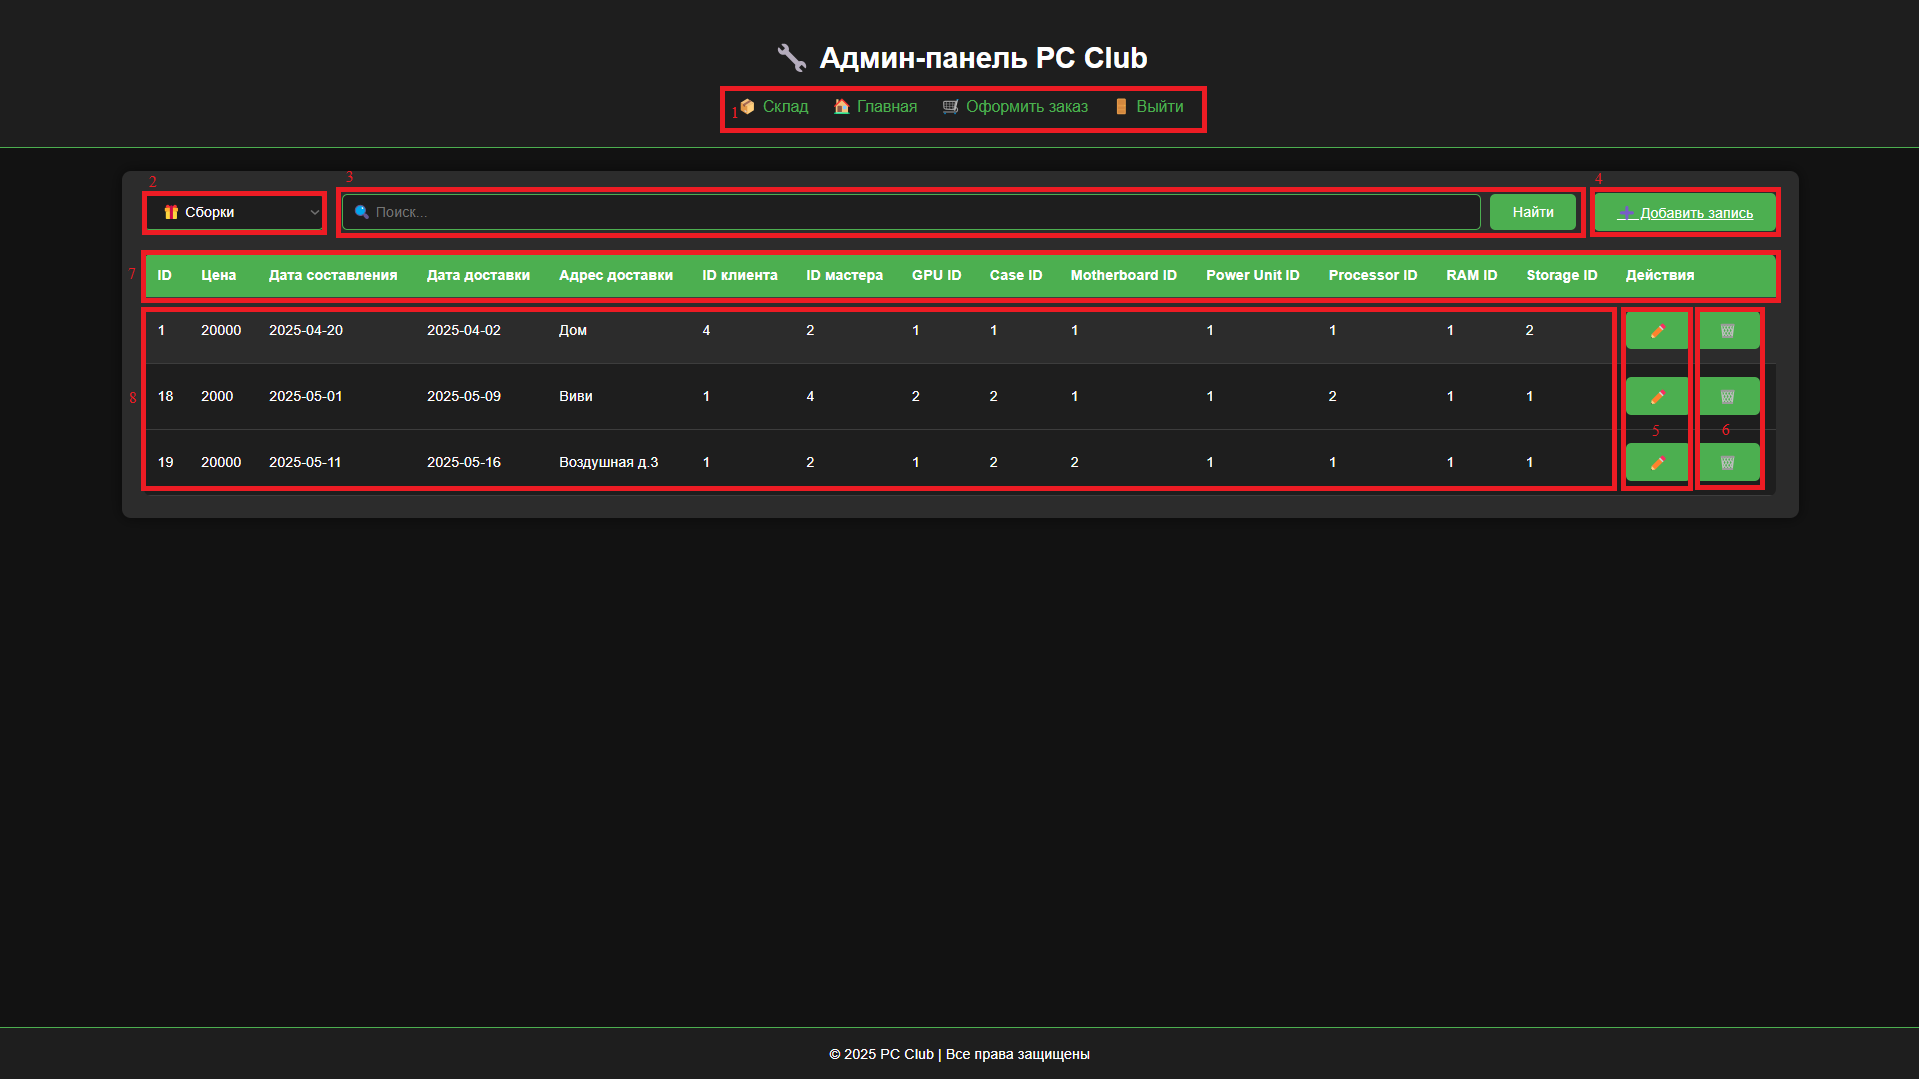
\includegraphics[width=1\linewidth]{adminall}}
\caption{Админ-панель Pc-Club общий вид}
\label{adminall:image}
\end{figure}

На рисунке \ref{razdeli:image} меню выбора между типом компонентов в панели админа.

\begin{figure}[htbp]
\center{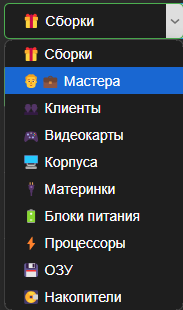
\includegraphics[width=0.25\linewidth]{razdeli}}
\caption{Разделы для каждого вида компонентов.}
\label{razdeli:image}
\end{figure}

На рисунке \ref{storedf:image} меню менеджмента склада для веб-приложения, здесь можно пополнять запасы недостающих комплектующих, потом применять их в заказах.

\begin{enumerate}
	\item Расширенная навигационная панель админа.
	\item Кнопка вызова меню выбора типа компонента.
	\item Ручной поиск по позициям и кнопка.
	\item Заголовок таблицы.
	\item Компонент из таблицы.
	\item Количество компонента на складе и поле для ввода нового значения.
	\item Кнопка для обновления значения.
\end{enumerate}

\begin{figure}[ht]
	\center{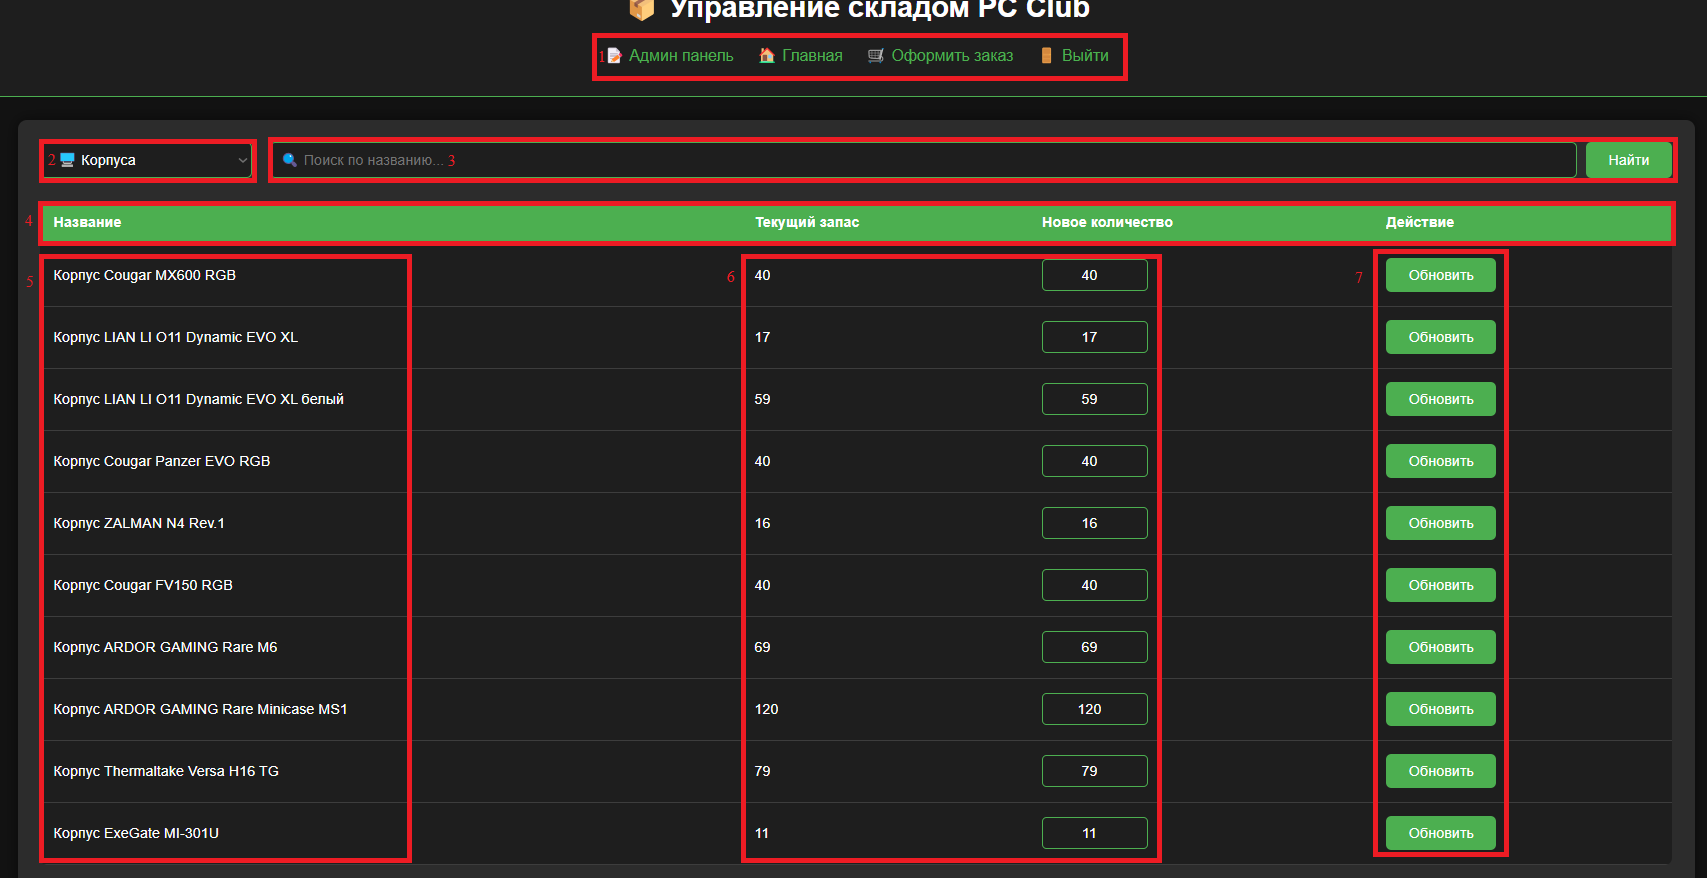
\includegraphics[width=1\linewidth]{storedf}}
	\caption{Страничка склада корпусов в качестве примера.}
	\label{storedf:image}
\end{figure}
\clearpage
